\chapter{Gradient Descent}

Gradient descent is a first-order iterative optimization algorithm for finding a local minimum of a differentiable function. The idea is to take repeated steps in the opposite direction of the gradient of the function at the current point, because this is the direction of steepest descent. Conversely, stepping in the direction of the gradient will lead to a local maximum of that function; the preocedure is then known as \textbf{gradient ascent}.

\section{Notation}
Let's introduce some convenient notation. The indicator function is a function for turning \texttt{true} and \texttt{false} answers into numbers or counts:
\begin{equation}
    1[x] = \begin{cases}
        1\qquad &\text{if }x=\texttt{true}\\
        0\qquad &\text{if }x=\texttt{false}\\
    \end{cases}
\end{equation}
We use a \textbf{vector notation}. We represent an example \(f_1,f_2,...,f_m\) as a single vector, \(\vec{x}\). Similarly, we can represent the weight \(w_1,w_2,...,w_m\) as a single vector, \(\vec{w}\).

The dot-product between two vectors \(\vec{a}\) and \(\vec{b}\) is defined as:
\begin{equation}
    a \cdot b = \sum_{j=1}^m a_jb_j
\end{equation}

\section{The optimization framework for Linear Models}
We have already seen the perceptron as a way of finding a weight vector \(\vec{w}\) and bias \(b\) that do a good job of separating positive training examples from negative training examples. The goal of the perceptron was to find a separating hyperplane for some training data set. Not all data sets are linearly separable. In the case that your training data \emph{isn't} linearly separable, you might want to find the hyperplane that makes the \emph{fewest errors} on the training data. We can write this down as a formal mathematics optimization problem as follows:
\begin{equation}
    \label{eqn:optimization}
    \min_{w,b} \sum_n 1[y_n(\vec{w} \cdot \vec{x} + b) > 0]
\end{equation}
The objective function is the thing we are trying to minimize. In this case, the objective function is simply the \textbf{error rate} of the linear classifier parametrized by \(\vec{w}\), \(b\).

We know that the perceptron algorithm is guaranteed to find parameters for this model if the data is linearly separable. In other words, if the optimum of \ref{eqn:optimization} is zero, then the perceptron will efficiently find parameters for this model.

\section{Convex Surrogate Loss Functions}
There are two equivalent definitions of a convex function. The first is that it's second derivative is always non-negative. The second definition is that any chord of the function lies above it.

Convex functions are nice because they are easy to minimize. This leads to the idea of \textbf{convex surrogate loss functions}. Since zero/one loss is hard to optimize, we want to optimize something else, instead. Since convex functions are easy to optimize, we want to approximate zero/one loss with a convex function. This approximating function will be called a \textbf{surrogate loss}. The surrogate losses we construct will always be \emph{upper bounds} on the true loss function: this guarantees that if you minimize the surrogate loss, you are also pushing down the real loss.

There are four common surrogate loss functions, each with their own properties:
\begin{align}
    \text{Zero/one}& \qquad l^{(0/1)}(y,\hat{y}) = 1[y\hat{y} \leq 0] \\
    \text{Hinge}& \qquad l^\text{(hin)}(y,\hat{y}) = \max\{0,1-y\hat{y}\} \\
    \text{Logistic:}& \qquad l^\text{(log)}(y,\hat{y}) = \frac 1 {\log 2} \log (1 + exp [-y\hat{y}]) \\
    \text{Exponential:}& \qquad l^\text{(exp)}(y,\hat{y}) = exp[-y\hat{y}] \\
    \text{Squared:}& \qquad l^\text{(sqr)}(y,\hat{y}) = (y-\hat{y})^2
\end{align}

There are two big differences in these loss functions. The first is how \emph{upset} they get by erroneous predictions. In the case of hinge and logistic loss, the growth of the function as \(\hat{y}\) goes negative is linear. For squared and exponential loss, it is super-linear. This means that exponential loss would rather get a few examples a little wrong than one example really wrong.
The other difference is how they deal with very confident correct predictions. Once \(y\hat{y}>1\), hinge loss does not care any more, but logistic and exponential loss still think you can do better. On the other hand, squared loss thinks it's just as bad to predict \(+3\) on a positive example as it is to predict \(-1\) on a positive example.

\begin{figure}[t]
\begin{center}
    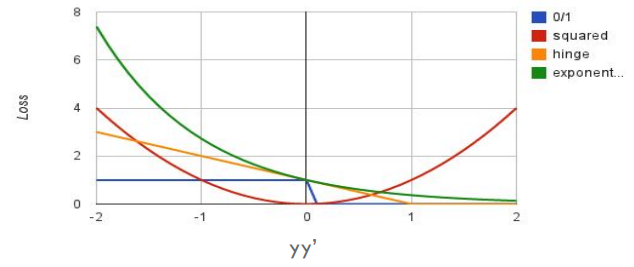
\includegraphics[width=\textwidth]{039}
    \vspace*{-25pt}
\end{center}
\caption{Surrogate loss functions}
\label{fig:039}
\end{figure}

\section{Gradients, math review}
A gradient is a multidimensional generalization of a derivative. Suppose you have a function \(f : \mathbb{R}^D \to \mathbb{R}\) that takes a vector \(\vec{x} = \langle x_1, x_2, ..., x_D \rangle \) as input and produces a scalar value as output.

You can differentiate this function according to any one of the inputs; for instance, you can compute \(\frac {\delta f} {\delta x_5}\) to get the derivative with respect to the fifth input. The \textbf{gradient} of \(f\) is just the vector consisting of the derivative \(f\) with respect to each of its input coordinates independently, and is denoted \(\nabla f\), or, when the input to \(f\) is ambiguous, \(\nabla_x f\). This is defined as:
\begin{align}
    \nabla_x f = \left\langle \frac{\delta f}{\delta x_1}, \frac{\delta f}{\delta x_2}, ..., \frac{\delta f}{\delta x_D} \right\rangle
\end{align}
For example, consider the function \(f(x_1,x_2,x_3) = x_1^3+5x_1x_2-3x_2x_3^2\). The gradient is:
\begin{align}
    \nabla_x f = \langle 3x_1^2 + 5x_2, 5x_1-3x_3^2, -6x_2x_3 \rangle
\end{align}
Note that if \(f : \mathbb{R}^ \to \mathbb{R}\), then \(\nabla f : \mathbb{R}^D \to \mathbb{R}^D\). If you evaluate \(\nabla f(x)\), this will give you the gradient at \(\vec{x}\), a vector in \(\mathbb{R}^D\). This vector can be interpreted as the direction of \textbf{steepest ascent}: namely, if you were to traver an infinitesimal amount in the direction of the gradient, you would go uphill the most.

\section{Optimization with gradient descent}
Suppose you are trying to find the maximum of a function \(f(\vec{x})\). The optimizer maintains a current estimate of the parameter of interest, \(\vec{x}\). At each step, it measures the \textbf{gradient} of the function it is trying to optimize. This measurement occurs at the current location, \(\vec{x}\). Call the gradient \(\vec{g}\). It then takes a step in the direction of the gradient, where the size of the step is controlled by a parameter \(\eta\). The complete step is \(\vec{x} \gets \vec{x} + \eta \vec{g}\). This is the basic idea of \textbf{gradient ascent}.

\begin{wrapfigure}{l}{0.25\textwidth}
\begin{center}
    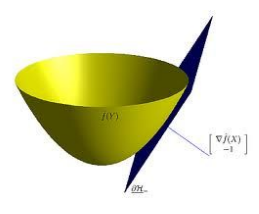
\includegraphics[width=0.25\textwidth]{038}
    \caption{Convex function}
	\vspace*{-40pt}
\end{center}
\label{fig:038}
\end{wrapfigure}

The opposite of gradient ascent is \textbf{gradient descent}. All of our learning problems will be framed as \emph{minimization} problems (trying to reach the bottom of a ditch, rather than the top of a hill). Therefore, descent is the primary approach you will use. One of the major conditions for gradient ascent being able to find the true, \textbf{global minimum}, of its objective function is convexity. Without convexity, all is lost.

\subsection{Algorithm}
\begin{algorithm}
    \caption{GradientDescent($F$, $K$, $\eta_1, ..., \eta_K$)}
    \label{alg:gradient_descent}
$\vec{z}^{(0)} = \langle 0,0,...,0 \rangle $\;
\For{$k \gets 1,...,K$}{
    $\vec{g}^{(k)} \gets \nabla_{\vec{z}} F |_{\vec{z}^{\,(k-1)}}$\;
    $\vec{z}^{(k)} \gets \vec{z}^{\,(k-1)} - \eta^{(k-1)} \vec{g}^{\,(k)}$\;
}
\Return{$\vec{z}^{\,(K)}$}
\end{algorithm}
The function takes as argument the function \(F\) to be minimized, the number of iterations \(K\) to run and a sequence of learning rates \(\eta_1, ..., \eta_K\). 

The only real work you need to do to apply a gradient descent method is be able to compute derivatives. Suppose we choose the exponential loss function. We are interested on how much we want to move in the error direction at each iteration: namely, we are interested on the value of \(\frac \delta {\delta w_i} l(z)\).
\begin{align}
    \label{eqn:loss_derivative}
    \frac {\delta l} {\delta w_j} &= \frac \delta {\delta w_j} \sum_{i=1}^n \exp (-y_i (w \cdot x_i + b)) \\
    &= \sum_{i=1}^n \exp (-y_i (w \cdot x_i + b)) \frac \delta {\delta w_j} -y_i (w \cdot x_i + b)
\end{align}
Now, in order to make it more clear, let's expand the operations for the member \(- \frac \delta {\delta w_i} y_i(w \cdot x_i + b)\).
\begin{align*}
    - \frac {\delta l} {\delta w_j} -y_j (w \cdot x_j + b) &= - \frac \delta {\delta w_j} y_j (\sum_{j=1}^m w_j x_{ij} + b)\\
    &= -\frac \delta {\delta w_j} y_j (w_1 x_{i1} + w_2 x_{i2} + ... + w_m x_{im} + b) \\
    &= -\frac \delta {\delta w_j} (y_j w_1 x_{i1} + y_j w_2 x_{i2} + ... + y_j w_m x_{im} + y_j b) \\
    &= -y_j x_{ij}
\end{align*}
Let's now take this result and return to expand the equation \ref{eqn:loss_derivative}.
\begin{align}
    \frac \delta {\delta w_j} &= \sum_{i=1}^n \exp (-y_i (w \cdot x_i + b)) \frac \delta {\delta w_j} -y_i (w \cdot x_i + b) \\
    &= \sum_{i=1}^n -y_i x_{ij} \exp (-y_i (w \cdot x_i + b))
\end{align}
That means that for each example \(x_i\), the \textbf{exponential update rule} is:
\begin{equation}
    w_j = w_j + \eta y_i x_{ij} exp(-y_i (w \cdot x_i + b))
\end{equation}
If you remember from Algorithm \ref{alg:perceptron} perceptron algorithm, there is a similarity: \(w_i \gets w_i + f_i*label\). In practice: \(w_j \gets w_j + x_{ij} y_i c\), where \(c = \eta exp(-y_i (w \cdot x_i + b))\).

\newpage
\begin{exercise}[topsep=20pt,itemsep=10pt]
    \ex[!] What is gradient descent?
    \ex What is the optimization framework for non linearly separable training data?
    \ex What is a convex surrogate loss function?
    \ex How can we perform optimization with gradient descent?
    \ex[!] Describe the update of the gradient descent, and the update rule with loss.
    \ex[!] How does the perceptron update? How does the gradient descent update?
\end{exercise}